%\documentclass[en,dissfinal,rgbcolor]{template/rrlab} % For final Dissertation
%\documentclass[en,diss,boldauthor]{template/rrlab}    % For initial submission phase of Dissertation
\PassOptionsToPackage{dvipsnames}{xcolor}
\documentclass[en,]{template/rrlab}

\RRLABtitle{Reinforcement Learning based Pretraining for Autonomous Bus Operation}

% Autor der Arbeit:
\RRLABauthor{Vedaant Joshi}

% Typ der Arbeit (z.B. Diplomarbeit, Projektarbeit, Seminararbeit,..):
\RRLABtype{Master Thesis}

% Datum der Ausgabe der Arbeit
\RRLABinception{17.07.2023}

% Datum der Abgabe der Arbeit
\RRLABsubmission{17.01.2023}

% Erster Gutachter
\RRLABfirstreviewer{Prof. Dr. Karsten Berns}

% Zweiter Gutachter
\RRLABsecondreviewer{Jakub Pawlak, M. Sc.}

%% Nur für Projekt-, Diplomarbeit, Bachelor-, Masterthesis
% Betreuer  
\RRLABsupervisor{Jakub Pawlak, M. Sc.}

\RRLABdegree{Doktor-Ingenieur (Dr.-Ing.)}

% Datum der Abgabe der Aussprache
\RRLABdefense{irgendwann}

% Prüfungsvorsitzender
\RRLABchair{irgendwer}

% Dekan
\RRLABdean{irgendwer}

%%%%%%%%%%%%%%%%%%%%%%%%%%%%%%%%%%%%%%%%%%%%%%%%%%%%%%%%%%%%
%% Einbinden von zusätzlichen Paketen 
%% Hier kann der geübte TeX-Benutzer weitere 
%% Pakete einbinden
%%
%% Bereits eingebundene Pakete in <rrlab.cls>
%% \usepackage[T1]{fontenc}  T1-encoded fonts: auch Wörter mit Umlauten trennen
%% \usepackage{lmodern}  Neuerer Ersatz für Schriftfamilie 'ae' (zusammen mit fontenc)
%% \usepackage{inputenc}  Eingabe nach ISO 8859-1 (Latin1)
%% \usepackage[final]{graphicx}  um Graphiken einzubinden
%% \usepackage{makeidx} wir wollen auch einen Index
%% \usepackage{geometry}  Seitenränder einstellen leichtgemacht
%% \usepackage{fancyhdr}  definiere einfache Headings
%% \usepackage{longtable}  seitenübergreifende Tabellen
%% \usepackage{booktabs}  fuer spezielle unterteilungslinien
%% \usepackage[T1]{url}  zum Darstellen von URLs, zusätzlich werden Zeilenumbrüche in URLs ermöglicht
%% \usepackage{caption}  die Schriftgröße für Captions ist small, die Labels sind zusätzlich fett
%% \usepackage{subcaption}  für subfigure environment (Ersatz für subfig)
%% \usepackage[tight,nice]{units}  Typografisch korrekte Darstellung von Einheiten
%% \usepackage{listings}  Einbindung und Darstellung von Quellcode
%% \usepackage{multibib}  Unterstützung von mehreren Bibliografien
%% \usepackage{microtype}  Typografische Erweiterungen
%% \usepackage{xcolor}  Farbkodierung für Bildschirm (RGB)
%% \usepackage{amssymb,amsmath,dsfont}  Mathematikumgebung und -symbole
%% \usepackage{ifthen}  ifthenelse Syntax
%% \usepackage{datetime}  Erweiterter Zugriff auf Datums- und Zeitwerte
%%%%%%%%%%%%%%%%%%%%%%%%%%%%%%%%%%%%%%%%%%%%%%%%%%%%%%%%%%%%
%% einige weitere Pakete, die evtl. nützlich sein können
%% \usepackage{tikz}  Tik Z ist kein Zeichenprogramm! Es ist die benutzfreundliche Schnittstelle zu PGF.
%% \usetikzlibrary{shapes,arrows,calc,patterns,fit}  zusätzliche Bibliothek zu tikz
%% \usepackage{pgfplots}  interface um pgf plots in tex darzustellen
%% \usepackage{lscape}  landscape-Paket um text um 90° zu rotieren
%% \usepackage{rotating}  um Bilder zu drehen
%% \usepackage{marvosym}  einige zusätzliche symbole
%% \usepackage{textcomp}  weitere symbole
%% \usepackage{eurosym}  Euro-Symbol


%%%%%%%%%%%%%%%%%%%%%%%%%%%%%%%%%%%%%%%%%%%%%%%%%%%%%%%%%%%%
%% Makrodefinitionen. 
%% Hier kann der geübte TeX-Benutzer eigene Makros oder
%% Kommandos definieren
%%
%% Für häufig verwendete Namen sind einige Makros vordefiniert,
%% siehe template/rrlab_macros.tex
%%%%%%%%%%%%%%%%%%%%%%%%%%%%%%%%%%%%%%%%%%%%%%%%%%%%%%%%%%%%


%%%%%%%%%%%%%%%%%%%%%%%%%%%%%%%%%%%%%%%%%%%%%%%%%%%%%%%%%%%%
%% Bilderverzeichnisse. 
%% Die hier angegebenen Verzeichnisse werden neben dem 
%% aktuellen Verzeichnis nach Bilddateien durchsucht.
%%%%%%%%%%%%%%%%%%%%%%%%%%%%%%%%%%%%%%%%%%%%%%%%%%%%%%%%%%%%
\graphicspath{%
 {./bilder/}
}

%%%%%%%%%%%%%%%%%%%%%%%%%%%%%%%%%%%%%%%%%%%%%%%%%%%%%%%%%%%%
%% Document Environment. 
%% Hier geht's dann wirklich los.
%%%%%%%%%%%%%%%%%%%%%%%%%%%%%%%%%%%%%%%%%%%%%%%%%%%%%%%%%%%%
\begin{document}
% Die folgenden Befehle nach Bedarf benutzen oder auskommentieren:

% Titelblatt generieren. Als Parameter kann z.B. ein Bild oder
% zusätzlicher Text angegeben werden. Das erscheint dann in der 
% Mitte des Titelblattes. Ausserdem wird das Datum übergeben:
% Bei Dissesrtationen taucht weder Titelbild noch Datum auf!!
\RRLABtitlepage{}{\currentdate\today}


% Zweite Seite mit Titel, Autor, Betreuer etc.
\RRLABsecondpage


% Seite mit der Erklärung, die Arbeit selbständig verfasst zu haben:
% Parameter ist das Datum, an dem die Erklärung unterschrieben wird
\RRLABdeclaration{\currentdate\today}

\RRLABabstract{Abstract}{

}

\RRLABcontents
\chapter{Introduction}
The report is structured as follows: In Section \ref{technical_background}, we dive into the essential technical background knowledge necessary to understand the thesis's objectives. Section \ref{related_work} offers a brief overview of prior methods used as a pretraining method for object detection. Next, Section \ref{concept_implementation} outlines the methodology applied in this thesis. Section \ref{experiments} presents a comprehensive examination of the experiments conducted during this research and the resultant findings. Finally, Section \ref{discussion_conclusion} engages in a detailed discussion of the outcomes derived from analyzing the experimental data, culminating in the conclusion.


\chapter{Technical Background} \label{technical_background}
In this chapter, we present a comprehensive study of the concepts of Artificial Intelligence (AI), Machine Learning (ML), and Deep Learning (DL). The content covered under this chapter will serve as the essential concepts necessary for understanding the implementation of the Reinforcement Learning algorithm and Object Detection methodologies.

The term "Artificial Intelligence" was coined by John McCarthy \cite{dartmouth}, an American computer scientist. He is considered one of the ground-breakers in the field of AI. Since then, many advancements have occurred in the field of AI. The basic goal of an AI software is to find patterns in large amount of data provided to it and then make a decision in a way humans generally would. Generally, a human supervision is required to check if the decision taken by the system are in accordance, but some AI systems have been designed to work without human supervision. An example of this is found in Autonomous Driving Systems, where the system uses various sensors to gather data from the the environment and make decisions with the aim of fulfilling the goal while following all the safety measures. In subsequent subsections, we will look into subsets of AI. The relation between AI, Machine Learning, Neural Networks and Deep learning is shown in Figure \ref{fig:chapter-2_ai_ml_dl}

\begin{figure}[ht]
    \centering
    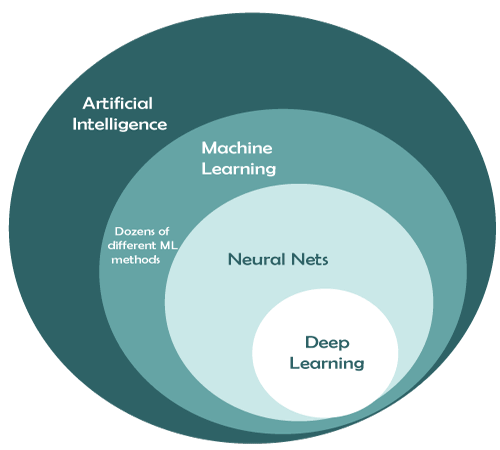
\includegraphics[height=0.5\textwidth]{figures/deep-learning-vs-machine-learning-vs-artificial-intelligence1.png}
    \caption{Relation between AI, Machine Learning, Neural Networks and Deep Learning.}
    \cite{ai-ml-dl, https://www.researchgate.net/figure/Relationship-between-artificial-intelligence-machine-learning-neural-network-and-deep_fig3_354124420}
    \label{fig:chapter-2_ai_ml_dl}
\end{figure}

\section{Machine Learning}
Machine Learning (ML) is a sub-field of Artificial Intelligence with numerous application across different domains, but for every application the underlying concept which ML systems uses is to enhance the performance of the system as more data is given to it overtime. The objective of a Machine Learning system is to be able to mimic Human behaviour in such a way that it learns the hidden patterns present in the given dataset, allowing the system to make predictions with high accuracy for given similar unseen inputs. There are different categories of Machine Learning, which are divided into groups based on the type of dataset provided during the training. When a dataset consists of both the data point, represented by its selected features, and the corresponding label, which assigns a category to that data point, this method is called as Supervised Learning. Few notable types of Supervised Learning are Regression, Classification, Naive Bayes, Neural Networks, and Random Forest. In Unsupervised Machine Learning, the data is unlabelled. The algorithm analyzes the data points to gain insight from the hidden features and clusters the similar data points together. K-means clustering, K-Nearest Neighbour, Principal Component Analysis and Singular Value Decomposition fall under the category of Unsupervised ML Algorithms. Combining both of the aforementioned methods, third ML method is known as Semi-Supervised Learning, where the dataset contains of small amount of labelled data points and more number of unlabelled data points.This particular method is proved to be useful when it is difficult to obtain enough labelled data to train the algorithm, so both unlabelled and labelled data points are used.Finally, the last category of ML which will be primary focus of this read is Reinforcement Learning(RL). RL is reward-based algorithm that learns to interact with the environment iteratively, and is rewarded positive or negative rewards based on the actions/decisions taken by the systems. Detailed introduction to all the types of ML algorithm are explained in the following subsections. 

\subsection{Supervised Learning}
Supervised Machine Learning algorithms are given labelled data as input. It is called as supervised, as explicitly the category of each data point is available and while training it iteratively the labels are treated as the ground truth to verify if the ML system has accurately categorized the data point. In accordance of the ground truth and the predicted output, the parameters of the network are updated in such a way that the accuracy of the system increases over time. The assessment of the system is done during the testing phase, by feeding previously unseen data points (never used during training phase). Further, Supervised Learning is divided into two categories. This is based on the type of the task the system is designed to perform \cite{SML}. Figure shows the depicting of SML models working. (Add a figure showing two classes with different color in one graph and adjacent graph a line diving the data-points)

\paragraph{Regression}
In Regression based Supervised Learning, the parameters of the model are updated in such a way that it finds a best line fitting all the data points. Fitting the data points means to minimize the distance between the line and each individual data point. Achieving this, results into making accurate predictions for future unseen instances. Here, the labels are continuous values. For instance, predicting Monthly Sales based on input features such as money spend on advertising. This allows the model to be trained using historical data, which then helps in approximating Monthly Sales for the current month and also future upcoming sales

\paragraph{Classification}
In contrast to Regression Supervised Learning, Classification-based Supervised Learning involves discrete classes. The model's objective is to assign a single class to each data point, determined by the features of the input data point. During the training phase, the model output and ground truth labels are compared, and the model parameters are adjusted based on the differences between the labels over multiple iterations. One such example is of spam email detection. The emails can be classified into two categories : "spam" or "not spam". The input features given to the model can be certain word occurrences, fishy email address, or presence of unnecessary links.

\subsection{Unsupervised Learning}\label{unsupervised-learning}
The difference between Supervised Learning and Unsupervised Learning is absence of Labels which is visually described in Figure \ref{fig:chapter-2_sup_vs_unsup}. The algorithm's objective is to learn the underlying pattern. The entire dataset follows a pattern that needs to be identified by the algorithm, and based on that, similar points are clustered together. After the clustering of all the data points is complete, one can observe that if two data points are picked from the same cluster, their properties/features will be similar. In contrast, if two points from different clusters are chosen, there will be notable differences between the features. There are two types of clustering; namely, Clustering, Dimensionality Reduction and Association.

\begin{figure}[ht]
    \centering
    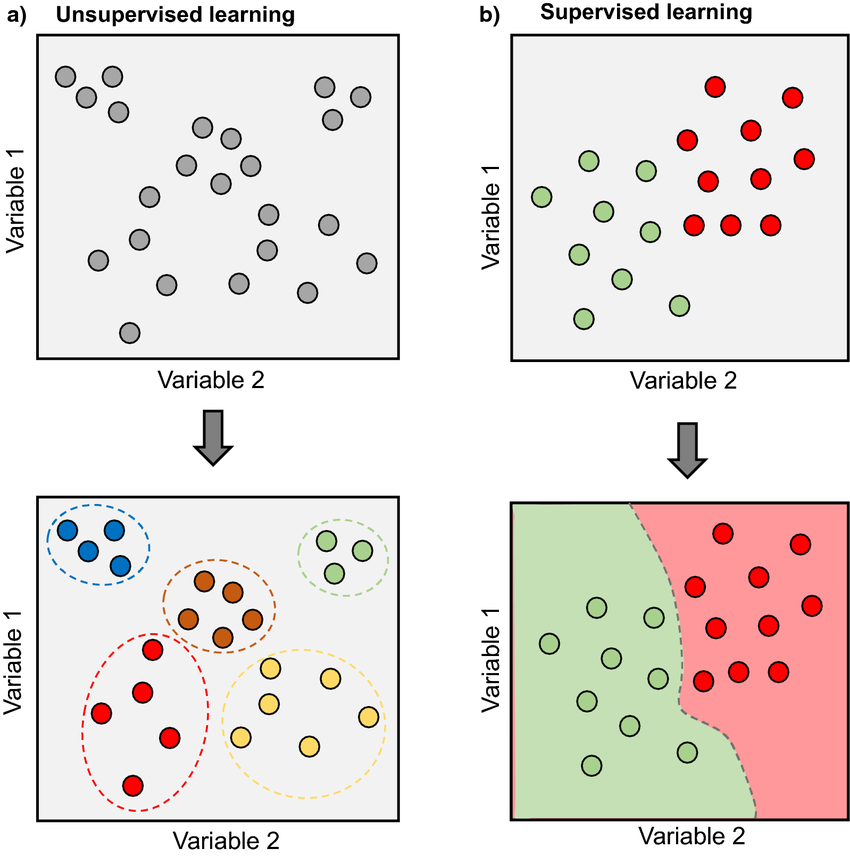
\includegraphics[height=0.5\textwidth]{figures/Supervised-and-unsupervised-machine-learning-a-Schematic-representation-of-an.png}
    \caption{Difference between Supervised and Unsupervised Machine learning algorithms}
    \cite{sup_vs_unsup}
    \label{fig:chapter-2_sup_vs_unsup}
\end{figure}

\paragraph{Clustering}
In simple terms, clustering involves grouping similar data points together into clusters. As discussed in \ref{unsupervised-learning}, data points with similar characteristics form one cluster, while those with different features or properties make up another. When a new data point is introduced to the system, it is assigned to a cluster based on its features. One commonly used clustering algorithm is the K-means algorithm \cite{Jin2010}. This algorithm suggests that, starting with an initial clustering that is not optimal, each point is moved to its nearest new center (mean). The cluster center is then updated by calculating the mean of the members of that cluster. This process is iterated until the mean of each cluster no longer changes. 

\paragraph{Dimensionality Reduction}
Dimensionality Reduction (DR) is the process of removing redundant features, noisy and irrelevant data, to improve learning feature accuracy and reduce the training time \cite{DR}. This techniques have been implemented using feature selection and extraction method. Principal Component Analysis (PCA) is one of the DR technique which reduces the learning process time. 

\paragraph{Association}
Association or Association Rule Mining finds interesting associations in large sets of data items \cite{Cios2007}. One of the most used application is of Market-Basket analysis, where it analyzes customer buying patterns by finding relation between items that customers put together. This knowledge then can be used by the seller to make profits over time.

\subsection{Semi-Supervised Learning}
    Semi-Supervised is a kind of learning process where the algorithm takes advantage of both labeled dataset and unlabeled dataset. Labeled dataset contains those data points where the ground truth is available and unlabeled dataset lacks explicit labels. During the training process, the labeled data guides the learning process whereas for unlabeled data points the algorithm is required to find out the underlying patterns in that data set. This method is used when it becomes very expensive to acquire labeled dataset. It takes benefits from both concepts (Supervised and Unsupervised). The training process consist of training the base model with labeled data first, like in supervised learning. Thereafter, train the previously trained base model with unlabeled data to get pseudo labels. The pseudo labels with prediction confidence higher than a give threshold are added to the pool of labeled dataset. Then the new dataset formed is used to train the model. This can happen for several iterations and can improve the performance of the model iteratively. This can go other way round as well if the pseudo labels generated are incorrect and then model is trained on the basis of data points with incorrect labels.

\subsection{Reinforcement Learning}
Reinforcement Learning (RL) algorithms differs from the previous approaches. RL serves as a general framework for building systems that do not require human supervision to make decisions in order to perform a task \cite{buffet2020reinforcement}. The RL agent faces sequential decision-making problem. It interacts with the environment, which leads to reaching a particular state. Based on that current state, the agent has to make a decision of performing an action, resulting in changes to the environment that, in turn results into change in the current state and a reward is provided as a feedback for the action taken. In RL algorithm, the agent needs to learn to take good actions based on observations and rewards received. In-depth discussion on this topic is provided in Section \ref{rf}.

\section{Deep Learning}
Before diving deeper into the major concepts of Deep Learning, let us explore its backbone called as Neural Networks. Neural Network is a computational model which was inspired by the functioning and structuring of neurons present in human brain. The major components of a Neural Network are nodes, connection between those nodes, input layer, hidden layer(s) and finally an output layer. The input layer takes training and testing data points. After the initial input layer processes the input it is being forwarded to the hidden layer(s), where each layer extracts features and passes them further to other hidden layers. Every node in an layer are interconnected with nodes in previous and next layer. Before passing the features to the next layer, it is passed through Activation function. Basically, activation function adds non-linearity to the model (further discussed in Section \ref{activation_function}). The interconnected nodes consist of weights (some numerical values). Those weights are trainable parameters, which are trained over the period of multiple epochs. These weights are updated in a way that the loss between ground truth and the predicted computations is minimized.

Deep Learning or also called as Deep Neural Networks is the term used for the Neural Networks with multiple layers. Increasing the layers in a Neural Network enables learning of hidden patterns present in the input data distribution. Hence, Deep Learning is able to give accurate results on various different applications. The term itself was proposed in 1986 by Rina Dechter Dechter although the history of its appearance is tricky \cite{Deepl}. The very first general working learning algorithm consisting of supervised, deep, feedforward, multilayer perceptron was published by Alexey Ivakhnenko and Lapa in 1967 \cite{ivakhnenko1967cybernetics}. In 1989, Yann LeCun showed how to use a big back-propagation method for the first time in image recognition. He combined it with Convoltional Neural Networks to identify "handwritten" digits \cite{LeCun1989BackpropagationAT}. Significant progress was made after that in the coming years. In 1995, Support Vector Machine was developed by Dana Cortes and Vladimir Vapnik \cite{cortes1995support}. The application of Deep Neural Networks is mainly divided into two parts, namely, Computer Vision and Textual-based Application. The main point in history which can be considered as the turning point in the field of vision was the introduction of AlexNet (which uses Convolutional Neural Networks; further discussed in Section \ref{CNN}) \cite{NIPS2012_c399862d} by Alex K. et al. . It achieved notable success in the ImageNet Large Scale Visual Recognition Challenge (ILSVRC) in 2012, demonstrating the huge scope of using Deep Neural Networks in the field of image classification. In the field of textual-based data, introduction of Transformers \cite{vaswani2023attention}, Long-Short Term Memory (LSTM) \cite{LSTM}, Gated Recurrent Unit (GRU) \cite{GRU} and currently Large Language Models (LLM) \cite{LLM} are widely used. 

\subsection{Activation Function }\label{activation_function}
\subsection{Convolutional Neural Networks}\label{CNN}


\section{Reinforcement Learning}\label{rf}

\chapter{Related Work} \label{related_work}
\chapter{Concept and Implementation} \label{concept_implementation}
\chapter{Experiments and Results} \label{experiments}
\chapter{Discussion and Conclusion} \label{discussion_conclusion}


\RRLABbibliography{literatur}

\chapter{Appendix} \label{appendix}


%%%%%%%%%%%%%%%%%%%%%%%%%%%%%%%%%%%%%%%%%%%%%%%%%%%%%%%%%%%%
%% index generieren? ggf. auskommentieren
%%%%%%%%%%%%%%%%%%%%%%%%%%%%%%%%%%%%%%%%%%%%%%%%%%%%%%%%%%%%
% \RRLABindex

%%%%%%%%%%%%%%%%%%%%%%%%%%%%%%%%%%%%%%%%%%%%%%%%%%%%%%%%%%%%
%% Ende des Dokuments
%%%%%%%%%%%%%%%%%%%%%%%%%%%%%%%%%%%%%%%%%%%%%%%%%%%%%%%%%%%%
\end{document}
